% =============================================================================
%  Supporting Information for jcim.tex (J. Chem. Inf. Model.). Compile si.tex BEFORE jcim.tex:
%  the manuscript imports the S-numbered labels of this document through xr.
% =============================================================================
\documentclass[journal=jcisd8,manuscript=suppinfo]{achemso}
\usepackage[T1]{fontenc}
\usepackage{amsmath,amssymb}
\usepackage{booktabs}
\usepackage{array}
\usepackage{graphicx}
\usepackage{siunitx}
\usepackage{xcolor}
\usepackage[section]{placeins}
\usepackage{hyperref}
\usepackage[capitalise]{cleveref}
% Macros compartidas por jcim.tex (manuscrito) y si.tex (Supporting Information).
% Todas las cifras proceden de los ficheros numeros*.tex generados por los scripts; no se escriben a mano.
% Generado por hacer_numeros.py a partir de resultados/preliminar.json. No editar a mano.
\newcommand{\nShort}{6{,}137}
\newcommand{\nLong}{133}
\newcommand{\nTotal}{6{,}270}
\newcommand{\betaShortMed}{0.43}
\newcommand{\betaShortLo}{0.26}
\newcommand{\betaShortHi}{0.60}
\newcommand{\betaShortSubPct}{97.8}
\newcommand{\betaShortDiffPct}{0.03}
\newcommand{\betaShortDiffN}{2}
\newcommand{\betaLongMed}{0.65}
\newcommand{\betaLongLo}{0.49}
\newcommand{\betaLongHi}{0.83}
\newcommand{\betaLongSubPct}{69.2}
\newcommand{\betaLongDiffPct}{3.8}
\newcommand{\betaLongDiffN}{5}
\newcommand{\epSd}{0.19}
\newcommand{\epFactor}{1.21}
\newcommand{\epOutOnePointFivePct}{5.4}
\newcommand{\epOutTwoPct}{0.2}
\newcommand{\epRho}{0.92}
\newcommand{\ratioHalf}{8.86}
\newcommand{\ratioHalfLo}{4.70}
\newcommand{\ratioHalfHi}{12.47}
\newcommand{\rhoHalf}{0.91}
\newcommand{\withinHalfPct}{0.0}
\newcommand{\ratioOne}{5.23}
\newcommand{\ratioOneLo}{3.12}
\newcommand{\ratioOneHi}{7.26}
\newcommand{\rhoOne}{0.92}
\newcommand{\withinOnePct}{0.0}
\newcommand{\ratioTwo}{3.34}
\newcommand{\ratioTwoLo}{2.15}
\newcommand{\ratioTwoHi}{4.32}
\newcommand{\rhoTwo}{0.94}
\newcommand{\withinTwoPct}{0.0}
\newcommand{\ratioFive}{1.95}
\newcommand{\ratioFiveLo}{1.47}
\newcommand{\ratioFiveHi}{2.40}
\newcommand{\rhoFive}{0.96}
\newcommand{\withinFivePct}{0.8}
\newcommand{\ratioTen}{1.40}
\newcommand{\ratioTenLo}{1.18}
\newcommand{\ratioTenHi}{1.63}
\newcommand{\rhoTen}{0.98}
\newcommand{\withinTenPct}{16.5}
\newcommand{\ratioFifteen}{1.19}
\newcommand{\ratioFifteenLo}{1.08}
\newcommand{\ratioFifteenHi}{1.31}
\newcommand{\rhoFifteen}{0.99}
\newcommand{\withinFifteenPct}{73.7}
\newcommand{\ratioTwenty}{1.07}
\newcommand{\ratioTwentyLo}{1.03}
\newcommand{\ratioTwentyHi}{1.12}
\newcommand{\rhoTwenty}{1.00}
\newcommand{\withinTwentyPct}{100.0}
\newcommand{\nPairs}{133}
\newcommand{\PairEndRatio}{2.90}
\newcommand{\PairEndLo}{1.58}
\newcommand{\PairEndHi}{4.74}
\newcommand{\PairEndRho}{0.84}
\newcommand{\PairEndRecall}{85}
\newcommand{\PairAvgRatio}{3.90}
\newcommand{\PairAvgLo}{2.14}
\newcommand{\PairAvgHi}{6.22}
\newcommand{\PairAvgRho}{0.85}
\newcommand{\PairAvgRecall}{81}
\newcommand{\nLongLit}{37}
\newcommand{\nLongScreen}{96}
\newcommand{\nRep}{94}
\newcommand{\sdLong}{0.98}
\newcommand{\RepEndRho}{0.48}
\newcommand{\RepEndFactor}{1.43}
\newcommand{\RepEndSd}{0.35}
\newcommand{\RepEndDiffPct}{38}
\newcommand{\RepEndIcc}{0.47}
\newcommand{\RepEndSdAll}{0.49}
\newcommand{\RepEndSdSub}{0.44}
\newcommand{\RepAvgRho}{0.56}
\newcommand{\RepAvgFactor}{1.32}
\newcommand{\RepAvgSd}{0.28}
\newcommand{\RepAvgDiffPct}{32}
\newcommand{\RepAvgIcc}{0.58}
\newcommand{\RepAvgSdAll}{0.43}
\newcommand{\RepAvgSdSub}{0.40}
\newcommand{\RepBetaSd}{0.15}
\newcommand{\RepBetaRho}{-0.07}
\newcommand{\nPrefix}{133}
\newcommand{\valMaxDev}{5e-7}
\newcommand{\driftMed}{1.2}
\newcommand{\driftMax}{34}
\newcommand{\driftFracPct}{63}
\newcommand{\preEndRatioTwo}{4.43}
\newcommand{\preEndErrTwo}{4.43}
\newcommand{\preEndCovTwo}{1}
\newcommand{\preEndRatioFive}{2.83}
\newcommand{\preEndErrFive}{2.83}
\newcommand{\preEndCovFive}{3}
\newcommand{\preEndRatioTen}{2.02}
\newcommand{\preEndErrTen}{2.02}
\newcommand{\preEndCovTen}{14}
\newcommand{\preEndRatioTwenty}{1.43}
\newcommand{\preEndErrTwenty}{1.45}
\newcommand{\preEndCovTwenty}{47}
\newcommand{\preHalfRatioTwo}{6.39}
\newcommand{\preHalfErrTwo}{6.39}
\newcommand{\preHalfCovTwo}{0}
\newcommand{\preHalfRatioFive}{4.05}
\newcommand{\preHalfErrFive}{4.05}
\newcommand{\preHalfCovFive}{0}
\newcommand{\preHalfRatioTen}{2.55}
\newcommand{\preHalfErrTen}{2.55}
\newcommand{\preHalfCovTen}{2}
\newcommand{\preHalfRatioTwenty}{1.78}
\newcommand{\preHalfErrTwenty}{1.78}
\newcommand{\preHalfCovTwenty}{12}
\newcommand{\preFitRatioTwo}{2.83}
\newcommand{\preFitErrTwo}{2.85}
\newcommand{\preFitCovTwo}{23}
\newcommand{\preFitRatioFive}{2.02}
\newcommand{\preFitErrFive}{2.02}
\newcommand{\preFitCovFive}{39}
\newcommand{\preFitRatioTen}{1.48}
\newcommand{\preFitErrTen}{1.51}
\newcommand{\preFitCovTen}{56}
\newcommand{\preFitRatioTwenty}{1.16}
\newcommand{\preFitErrTwenty}{1.24}
\newcommand{\preFitCovTwenty}{78}
\newcommand{\prePowRatioTwo}{0.72}
\newcommand{\prePowErrTwo}{1.50}
\newcommand{\prePowCovTwo}{59}
\newcommand{\prePowRatioFive}{0.95}
\newcommand{\prePowErrFive}{1.37}
\newcommand{\prePowCovFive}{68}
\newcommand{\prePowRatioTen}{1.07}
\newcommand{\prePowErrTen}{1.26}
\newcommand{\prePowCovTen}{74}
\newcommand{\prePowRatioTwenty}{1.11}
\newcommand{\prePowErrTwenty}{1.20}
\newcommand{\prePowCovTwenty}{74}
\newcommand{\ruleBetaNineStopPct}{3}
\newcommand{\ruleBetaNineTime}{49.3}
\newcommand{\ruleBetaNineErr}{1.37}
\newcommand{\ruleBetaNineErrStop}{1.38}
\newcommand{\ruleBetaNineTimeStop}{26.8}
\newcommand{\ruleBetaEightStopPct}{19}
\newcommand{\ruleBetaEightTime}{44.6}
\newcommand{\ruleBetaEightErr}{1.39}
\newcommand{\ruleBetaEightErrStop}{1.39}
\newcommand{\ruleBetaEightTimeStop}{21.2}
\newcommand{\ruleCvTenStopPct}{2}
\newcommand{\ruleCvTenTime}{49.3}
\newcommand{\ruleCvTenErr}{1.37}
\newcommand{\ruleCvTenErrStop}{1.36}
\newcommand{\ruleCvTenTimeStop}{21.0}
\newcommand{\ruleCvTwentyStopPct}{80}
\newcommand{\ruleCvTwentyTime}{15.6}
\newcommand{\ruleCvTwentyErr}{1.79}
\newcommand{\ruleCvTwentyErrStop}{2.22}
\newcommand{\ruleCvTwentyTimeStop}{7.3}
\newcommand{\ruleCvPowStopPct}{24}
\newcommand{\ruleCvPowTime}{43.4}
\newcommand{\ruleCvPowErr}{1.04}
\newcommand{\ruleCvPowErrStop}{1.13}
\newcommand{\ruleCvPowTimeStop}{22.7}
\newcommand{\sensLongSubMinPct}{46}
\newcommand{\sensLongSubMaxPct}{81}
\newcommand{\sensLongDiffMinN}{0}
\newcommand{\sensLongDiffMaxN}{19}
\newcommand{\RepEndIccLo}{0.31}
\newcommand{\RepEndIccHi}{0.63}
\newcommand{\RepEndIccSub}{0.53}
\newcommand{\RepEndIccSubLo}{0.33}
\newcommand{\RepEndIccSubHi}{0.66}
\newcommand{\RepEndPairFactor}{1.65}
\newcommand{\RepEndPairFactorNinetyFive}{2.67}
\newcommand{\RepAvgIccLo}{0.45}
\newcommand{\RepAvgIccHi}{0.70}
\newcommand{\RepAvgIccSub}{0.62}
\newcommand{\RepAvgIccSubLo}{0.45}
\newcommand{\RepAvgIccSubHi}{0.74}
\newcommand{\RepAvgPairFactor}{1.48}
\newcommand{\RepAvgPairFactorNinetyFive}{2.16}
\newcommand{\PairEndRhoLo}{0.76}
\newcommand{\PairEndRhoHi}{0.90}
\newcommand{\PairEndRhoScreen}{0.68}
\newcommand{\PairEndRhoLit}{0.93}
\newcommand{\PairEndTopFiveK}{7}
\newcommand{\PairEndTopFiveHits}{7}
\newcommand{\PairEndTopTenK}{13}
\newcommand{\PairEndTopTenHits}{11}
\newcommand{\PairEndTopTwentyK}{27}
\newcommand{\PairEndTopTwentyHits}{23}
\newcommand{\PairAvgRhoLo}{0.77}
\newcommand{\PairAvgRhoHi}{0.90}
\newcommand{\PairAvgRhoScreen}{0.70}
\newcommand{\PairAvgRhoLit}{0.94}
\newcommand{\PairAvgTopFiveK}{7}
\newcommand{\PairAvgTopFiveHits}{6}
\newcommand{\PairAvgTopTenK}{13}
\newcommand{\PairAvgTopTenHits}{10}
\newcommand{\PairAvgTopTwentyK}{27}
\newcommand{\PairAvgTopTwentyHits}{22}

% Generado por referencias.py a partir de resultados/referencias.json. No editar a mano.
\newcommand{\refN}{133}
\newcommand{\refSlopeVsDapp}{0.70}
\newcommand{\refPowErrMin}{1.33}
\newcommand{\refPowErrMax}{1.45}
\newcommand{\refPowBiasMin}{0.83}
\newcommand{\refPowBiasMax}{1.06}
\newcommand{\refEndErrMin}{2.37}
\newcommand{\refEndErrMax}{3.27}
\newcommand{\refEndBiasMin}{2.37}
\newcommand{\refEndBiasMax}{3.27}
\newcommand{\refFitErrMin}{1.80}
\newcommand{\refFitErrMax}{2.33}
\newcommand{\refFitBiasMin}{1.73}
\newcommand{\refFitBiasMax}{2.33}
\newcommand{\refPowSlopeErrFive}{1.99}
\newcommand{\refPowSlopeRatioFive}{0.54}
\newcommand{\refBracketFivePct}{78}
\newcommand{\refPowSlopeErrTen}{1.52}
\newcommand{\refPowSlopeRatioTen}{0.68}
\newcommand{\refBracketTenPct}{73}
\newcommand{\refPowSlopeErrTwenty}{1.36}
\newcommand{\refPowSlopeRatioTwenty}{0.77}
\newcommand{\refBracketTwentyPct}{69}
\newcommand{\refEndSlopeErrFive}{4.01}
\newcommand{\refFitSlopeErrFive}{3.05}

% Generado por frontera.py a partir de resultados/frontera.json. No editar a mano.
\newcommand{\frN}{133}
\newcommand{\frSplits}{500}
\newcommand{\frMinFixEndOneFive}{20.0}
\newcommand{\frTestFixEndOneFive}{20.0}
\newcommand{\frMetFixEndOneFive}{97}
\newcommand{\frMinFixFitOneFive}{12.0}
\newcommand{\frTestFixFitOneFive}{12.0}
\newcommand{\frMetFixFitOneFive}{61}
\newcommand{\frMinFixPowOneFive}{2.0}
\newcommand{\frTestFixPowOneFive}{2.0}
\newcommand{\frMetFixPowOneFive}{59}
\newcommand{\frMinRegimeOneFive}{34.7}
\newcommand{\frTestRegimeOneFive}{35.2}
\newcommand{\frMetRegimeOneFive}{64}
\newcommand{\frMinPrecFitOneFive}{36.2}
\newcommand{\frTestPrecFitOneFive}{37.0}
\newcommand{\frMetPrecFitOneFive}{67}
\newcommand{\frMinPrecPowOneFive}{11.5}
\newcommand{\frTestPrecPowOneFive}{11.9}
\newcommand{\frMetPrecPowOneFive}{76}
\newcommand{\frMinFixEndOneThree}{30.0}
\newcommand{\frTestFixEndOneThree}{30.0}
\newcommand{\frMetFixEndOneThree}{84}
\newcommand{\frMinFixFitOneThree}{20.0}
\newcommand{\frTestFixFitOneThree}{20.0}
\newcommand{\frMetFixFitOneThree}{96}
\newcommand{\frMinFixPowOneThree}{10.0}
\newcommand{\frTestFixPowOneThree}{7.5}
\newcommand{\frMetFixPowOneThree}{45}
\newcommand{\frMinRegimeOneThree}{n/a}
\newcommand{\frTestRegimeOneThree}{n/a}
\newcommand{\frMetRegimeOneThree}{0}
\newcommand{\frMinPrecFitOneThree}{n/a}
\newcommand{\frTestPrecFitOneThree}{50.0}
\newcommand{\frMetPrecFitOneThree}{0}
\newcommand{\frMinPrecPowOneThree}{21.0}
\newcommand{\frTestPrecPowOneThree}{20.9}
\newcommand{\frMetPrecPowOneThree}{93}
\newcommand{\frMinFixEndOneTwo}{40.0}
\newcommand{\frTestFixEndOneTwo}{40.0}
\newcommand{\frMetFixEndOneTwo}{79}
\newcommand{\frMinFixFitOneTwo}{n/a}
\newcommand{\frTestFixFitOneTwo}{25.0}
\newcommand{\frMetFixFitOneTwo}{0}
\newcommand{\frMinFixPowOneTwo}{20.0}
\newcommand{\frTestFixPowOneTwo}{20.0}
\newcommand{\frMetFixPowOneTwo}{50}
\newcommand{\frMinRegimeOneTwo}{n/a}
\newcommand{\frTestRegimeOneTwo}{n/a}
\newcommand{\frMetRegimeOneTwo}{0}
\newcommand{\frMinPrecFitOneTwo}{n/a}
\newcommand{\frTestPrecFitOneTwo}{n/a}
\newcommand{\frMetPrecFitOneTwo}{0}
\newcommand{\frMinPrecPowOneTwo}{21.0}
\newcommand{\frTestPrecPowOneTwo}{21.1}
\newcommand{\frMetPrecPowOneTwo}{71}

% Generado por techo.py a partir de resultados/techo.json. No editar a mano.
\newcommand{\techoNRep}{94}
\newcommand{\techoNPairsScreen}{96}
\newcommand{\techoEndCorr}{0.69}
\newcommand{\techoEndCorrLo}{0.56}
\newcommand{\techoEndCorrHi}{0.79}
\newcommand{\techoEndRTwo}{0.47}
\newcommand{\techoEndRelTwo}{0.64}
\newcommand{\techoEndRelFour}{0.78}
\newcommand{\techoEndRepForEight}{5}
\newcommand{\techoEndSdDyn}{0.24}
\newcommand{\techoEndSdStruct}{0.26}
\newcommand{\techoEndFracStructPct}{55}
\newcommand{\techoEndFracStructLo}{31}
\newcommand{\techoEndFracStructHi}{72}
\newcommand{\techoEndShortPrefRatio}{1.00}
\newcommand{\techoEndHetRho}{-0.26}
\newcommand{\techoEndHetP}{0.01}
\newcommand{\techoEndSdSlow}{0.40}
\newcommand{\techoEndSdFast}{0.30}
\newcommand{\techoEndRecallOneTopFive}{38}
\newcommand{\techoEndRecallOneTopTen}{45}
\newcommand{\techoEndRecallOneTopTwenty}{56}
\newcommand{\techoEndRecallTwoTopFive}{49}
\newcommand{\techoEndRecallTwoTopTen}{56}
\newcommand{\techoEndRecallTwoTopTwenty}{64}
\newcommand{\techoEndRecallFourTopFive}{61}
\newcommand{\techoEndRecallFourTopTen}{66}
\newcommand{\techoEndRecallFourTopTwenty}{73}
\newcommand{\techoEndRecallOneTopTenLo}{36}
\newcommand{\techoEndRecallOneTopTenHi}{55}
\newcommand{\techoEndDynN}{96}
\newcommand{\techoEndJointN}{92}
\newcommand{\techoEndJointDiffCorr}{0.53}
\newcommand{\techoEndJointFracStructPct}{57}
\newcommand{\techoEndJointFracStructLo}{44}
\newcommand{\techoEndJointFracStructHi}{69}
\newcommand{\techoEndBatchRepRatio}{1.05}
\newcommand{\techoEndBatchRepP}{0.31}
\newcommand{\techoEndBatchRepRatioLo}{0.95}
\newcommand{\techoEndBatchRepRatioHi}{1.17}
\newcommand{\techoEndBatchPrefRatio}{1.00}
\newcommand{\techoEndBatchPrefP}{0.89}
\newcommand{\techoEndBatchPrefRatioLo}{0.93}
\newcommand{\techoEndBatchPrefRatioHi}{1.06}
\newcommand{\techoEndBatchSdOrig}{0.50}
\newcommand{\techoEndBatchSdRep}{0.53}
\newcommand{\techoEndBatchSdOther}{0.47}
\newcommand{\techoEndBatchLeveneP}{0.67}
\newcommand{\techoEndRelUncentred}{0.47}
\newcommand{\techoAvgCorr}{0.76}
\newcommand{\techoAvgCorrLo}{0.66}
\newcommand{\techoAvgCorrHi}{0.84}
\newcommand{\techoAvgRTwo}{0.58}
\newcommand{\techoAvgRelTwo}{0.73}
\newcommand{\techoAvgRelFour}{0.84}
\newcommand{\techoAvgRepForEight}{3}
\newcommand{\techoAvgSdDyn}{0.20}
\newcommand{\techoAvgSdStruct}{0.20}
\newcommand{\techoAvgFracStructPct}{51}
\newcommand{\techoAvgFracStructLo}{20}
\newcommand{\techoAvgFracStructHi}{69}
\newcommand{\techoAvgShortPrefRatio}{0.96}
\newcommand{\techoAvgHetRho}{-0.23}
\newcommand{\techoAvgHetP}{0.02}
\newcommand{\techoAvgSdSlow}{0.29}
\newcommand{\techoAvgSdFast}{0.26}
\newcommand{\techoAvgRecallOneTopFive}{45}
\newcommand{\techoAvgRecallOneTopTen}{52}
\newcommand{\techoAvgRecallOneTopTwenty}{61}
\newcommand{\techoAvgRecallTwoTopFive}{56}
\newcommand{\techoAvgRecallTwoTopTen}{63}
\newcommand{\techoAvgRecallTwoTopTwenty}{70}
\newcommand{\techoAvgRecallFourTopFive}{67}
\newcommand{\techoAvgRecallFourTopTen}{72}
\newcommand{\techoAvgRecallFourTopTwenty}{77}
\newcommand{\techoAvgRecallOneTopTenLo}{44}
\newcommand{\techoAvgRecallOneTopTenHi}{60}
\newcommand{\techoAvgDynN}{96}
\newcommand{\techoAvgJointN}{92}
\newcommand{\techoAvgJointDiffCorr}{0.51}
\newcommand{\techoAvgJointFracStructPct}{52}
\newcommand{\techoAvgJointFracStructLo}{33}
\newcommand{\techoAvgJointFracStructHi}{66}
\newcommand{\techoAvgBatchRepRatio}{1.04}
\newcommand{\techoAvgBatchRepP}{0.34}
\newcommand{\techoAvgBatchRepRatioLo}{0.96}
\newcommand{\techoAvgBatchRepRatioHi}{1.12}
\newcommand{\techoAvgBatchPrefRatio}{0.95}
\newcommand{\techoAvgBatchPrefP}{0.10}
\newcommand{\techoAvgBatchPrefRatioLo}{0.91}
\newcommand{\techoAvgBatchPrefRatioHi}{1.01}
\newcommand{\techoAvgBatchSdOrig}{0.45}
\newcommand{\techoAvgBatchSdRep}{0.46}
\newcommand{\techoAvgBatchSdOther}{0.41}
\newcommand{\techoAvgBatchLeveneP}{0.82}
\newcommand{\techoAvgRelUncentred}{0.58}

% Generado por asignacion.py a partir de resultados/asignacion.json. No editar a mano.
\newcommand{\alN}{6{,}137}
\newcommand{\alReps}{200}
\newcommand{\alKurt}{0.13}
\newcommand{\alShapiroP}{0.81}
\newcommand{\alUnifTopOneBOne}{32}
\newcommand{\alUnifTopOneBTwo}{52}
\newcommand{\alHalvingTopOneBTwo}{85}
\newcommand{\alBoundTopOneBTwo}{82}
\newcommand{\alUnifTopOneBFour}{67}
\newcommand{\alHalvingTopOneBFour}{90}
\newcommand{\alBoundTopOneBFour}{89}
\newcommand{\alEqTopOneUnifTwo}{1.1}
\newcommand{\alSavingTopOneUnifTwo}{1.7}
\newcommand{\alEqTopOneUnifThree}{1.2}
\newcommand{\alSavingTopOneUnifThree}{2.5}
\newcommand{\alEqTopOneUnifFour}{1.2}
\newcommand{\alSavingTopOneUnifFour}{3.2}
\newcommand{\alUnifTopFiveBOne}{41}
\newcommand{\alUnifTopFiveBTwo}{57}
\newcommand{\alHalvingTopFiveBTwo}{77}
\newcommand{\alBoundTopFiveBTwo}{77}
\newcommand{\alUnifTopFiveBFour}{70}
\newcommand{\alHalvingTopFiveBFour}{85}
\newcommand{\alBoundTopFiveBFour}{86}
\newcommand{\alEqTopFiveUnifTwo}{1.2}
\newcommand{\alSavingTopFiveUnifTwo}{1.7}
\newcommand{\alEqTopFiveUnifThree}{1.3}
\newcommand{\alSavingTopFiveUnifThree}{2.2}
\newcommand{\alEqTopFiveUnifFour}{1.5}
\newcommand{\alSavingTopFiveUnifFour}{2.7}
\newcommand{\alUnifTopTenBOne}{48}
\newcommand{\alUnifTopTenBTwo}{61}
\newcommand{\alHalvingTopTenBTwo}{73}
\newcommand{\alBoundTopTenBTwo}{75}
\newcommand{\alUnifTopTenBFour}{72}
\newcommand{\alHalvingTopTenBFour}{83}
\newcommand{\alBoundTopTenBFour}{84}
\newcommand{\alEqTopTenUnifTwo}{1.2}
\newcommand{\alSavingTopTenUnifTwo}{1.6}
\newcommand{\alEqTopTenUnifThree}{1.5}
\newcommand{\alSavingTopTenUnifThree}{2.0}
\newcommand{\alEqTopTenUnifFour}{1.8}
\newcommand{\alSavingTopTenUnifFour}{2.2}
\newcommand{\alBoundHomoTopTenBFour}{85}
\newcommand{\alSavingTopTenUnifFourEmpEnd}{2.2}
\newcommand{\alSavingTopTenUnifFourNormAvg}{2.4}
\newcommand{\alHalvingTopOneBOneQuarterEnd}{74}
\newcommand{\alBoundTopOneBOneQuarterEnd}{68}
\newcommand{\alHalvingTopOneBFourAvg}{84}
\newcommand{\alBoundTopOneBFourAvg}{89}
\newcommand{\alMCErrMax}{0.4}
\newcommand{\alMCErrMed}{0.1}
\newcommand{\alRelPlanLo}{0.31}
\newcommand{\alRelPlanHi}{0.62}
\newcommand{\alRelTrue}{0.47}
\newcommand{\alMisLoTopOneBTwo}{78}
\newcommand{\alMisLoTopOneBFour}{85}
\newcommand{\alMisLoSavingTopOne}{3.0}
\newcommand{\alMisHiTopOneBTwo}{83}
\newcommand{\alMisHiTopOneBFour}{90}
\newcommand{\alMisHiSavingTopOne}{3.2}
\newcommand{\alTwoStageTopOneBTwo}{80}
\newcommand{\alTwoStageTopOneBFour}{85}
\newcommand{\alTwoStageSavingTopOne}{3.2}
\newcommand{\alTwoStageFourkSavingTopOne}{3.0}
\newcommand{\alTwoStageEightkSavingTopOne}{3.2}
\newcommand{\alTrueLoSavingTopOne}{2.4}
\newcommand{\alTrueHiSavingTopOne}{3.2}
\newcommand{\alMisLoTopFiveBTwo}{76}
\newcommand{\alMisLoTopFiveBFour}{85}
\newcommand{\alMisLoSavingTopFive}{2.6}
\newcommand{\alMisHiTopFiveBTwo}{76}
\newcommand{\alMisHiTopFiveBFour}{86}
\newcommand{\alMisHiSavingTopFive}{2.6}
\newcommand{\alTwoStageTopFiveBTwo}{74}
\newcommand{\alTwoStageTopFiveBFour}{80}
\newcommand{\alTwoStageSavingTopFive}{2.4}
\newcommand{\alTwoStageFourkSavingTopFive}{2.4}
\newcommand{\alTwoStageEightkSavingTopFive}{1.9}
\newcommand{\alTrueLoSavingTopFive}{2.1}
\newcommand{\alTrueHiSavingTopFive}{2.9}
\newcommand{\alMisLoTopTenBTwo}{74}
\newcommand{\alMisLoTopTenBFour}{83}
\newcommand{\alMisLoSavingTopTen}{2.2}
\newcommand{\alMisHiTopTenBTwo}{74}
\newcommand{\alMisHiTopTenBFour}{83}
\newcommand{\alMisHiSavingTopTen}{2.1}
\newcommand{\alTwoStageTopTenBTwo}{71}
\newcommand{\alTwoStageTopTenBFour}{80}
\newcommand{\alTwoStageSavingTopTen}{1.8}
\newcommand{\alTwoStageFourkSavingTopTen}{1.8}
\newcommand{\alTwoStageEightkSavingTopTen}{1.3}
\newcommand{\alTrueLoSavingTopTen}{1.8}
\newcommand{\alTrueHiSavingTopTen}{2.5}

% Generado por validacion_asignacion.py. No editar a mano.
\newcommand{\valAlNRep}{94}
\newcommand{\valAlNCamp}{92}
\newcommand{\valAlExtra}{46}
\newcommand{\valAlBrierGainTen}{36}
\newcommand{\valAlCalSlopeTen}{1.10}
\newcommand{\valAlCalSlopeLoTen}{0.66}
\newcommand{\valAlCalSlopeHiTen}{2.27}
\newcommand{\valAlKTen}{9}
\newcommand{\valAlOnlyATen}{67}
\newcommand{\valAlBoundTen}{78}
\newcommand{\valAlRandomTen}{71}
\newcommand{\valAlBothTen}{78}
\newcommand{\valAlDiffLoTen}{-11}
\newcommand{\valAlDiffHiTen}{22}
\newcommand{\valAlBrierGainTwenty}{16}
\newcommand{\valAlCalSlopeTwenty}{0.63}
\newcommand{\valAlCalSlopeLoTwenty}{0.33}
\newcommand{\valAlCalSlopeHiTwenty}{1.36}
\newcommand{\valAlKTwenty}{18}
\newcommand{\valAlOnlyATwenty}{72}
\newcommand{\valAlBoundTwenty}{72}
\newcommand{\valAlRandomTwenty}{70}
\newcommand{\valAlBothTwenty}{72}
\newcommand{\valAlDiffLoTwenty}{-17}
\newcommand{\valAlDiffHiTwenty}{11}

% Generado por ml_demo.py a partir de resultados/ml_demo.json. No editar a mano.
\newcommand{\mlNSys}{6{,}042}
\newcommand{\mlFolds}{5}
\newcommand{\mlCorr}{0.71}
\newcommand{\mlCorrLo}{0.70}
\newcommand{\mlCorrHi}{0.72}
\newcommand{\mlRTwo}{0.50}
\newcommand{\mlFracCeilPct}{103}
\newcommand{\mlImplied}{1.03}
\newcommand{\mlImpliedLo}{1.01}
\newcommand{\mlImpliedHi}{1.00}
\newcommand{\mlRepN}{94}
\newcommand{\mlRepA}{0.67}
\newcommand{\mlRepB}{0.69}
\newcommand{\mlRepMean}{0.78}
\newcommand{\mlRepMeanExp}{0.79}
\newcommand{\mlRepGainLo}{0.07}
\newcommand{\mlRepGainHi}{0.13}
\newcommand{\mlLongN}{133}
\newcommand{\mlLongAllModel}{0.79}
\newcommand{\mlLongAllShort}{0.84}
\newcommand{\mlLongAllDiffLo}{-0.13}
\newcommand{\mlLongAllDiffHi}{0.02}
\newcommand{\mlLongAllN}{133}
\newcommand{\mlLongScreenModel}{0.67}
\newcommand{\mlLongScreenShort}{0.68}
\newcommand{\mlLongScreenDiffLo}{-0.12}
\newcommand{\mlLongScreenDiffHi}{0.13}
\newcommand{\mlLongScreenN}{96}
\newcommand{\mlLongLitModel}{0.67}
\newcommand{\mlLongLitShort}{0.93}
\newcommand{\mlLongLitDiffLo}{-0.47}
\newcommand{\mlLongLitDiffHi}{-0.12}
\newcommand{\mlLongLitN}{37}
\newcommand{\mlLeakN}{168}
\newcommand{\mlLeakTraj}{0.66}
\newcommand{\mlLeakSys}{0.68}

\IfFileExists{numeros_segmentos.tex}{% Generado por segmentos.py a partir de resultados/segmentos.json. No editar a mano.
\newcommand{\segN}{133}
\newcommand{\segEndFirst}{1.63}
\newcommand{\segEndFirstLo}{1.52}
\newcommand{\segEndFirstHi}{1.81}
\newcommand{\segEndFirstVsAll}{1.42}
\newcommand{\segEndFracFirstPct}{93}
\newcommand{\segEndSlope}{0.92}
\newcommand{\segEndFracNegSlopePct}{85}
\newcommand{\segEndWithinTen}{25}
\newcommand{\segEndWilcoxonP}{3.6\times10^{-22}}
\newcommand{\segEndFirstScreen}{1.80}
\newcommand{\segEndFirstLit}{1.28}
\newcommand{\segHalfFirst}{1.47}
\newcommand{\segHalfFirstLo}{1.37}
\newcommand{\segHalfFirstHi}{1.55}
\newcommand{\segHalfFirstVsAll}{1.32}
\newcommand{\segHalfFracFirstPct}{92}
\newcommand{\segHalfSlope}{0.94}
\newcommand{\segHalfFracNegSlopePct}{89}
\newcommand{\segHalfWithinTen}{20}
\newcommand{\segHalfWilcoxonP}{2.0\times10^{-22}}
\newcommand{\segHalfFirstScreen}{1.54}
\newcommand{\segHalfFirstLit}{1.30}
\newcommand{\segBetaFirst}{0.48}
\newcommand{\segBetaLate}{0.31}
\newcommand{\haySegmentos}{1}}{}
\DeclareSIUnit{\angstrom}{\text{\AA}}
\newcommand{\todo}[1]{\textcolor{orange!80!black}{[TODO: #1]}}
\newcommand{\Dapp}{D_{\mathrm{app}}}
\newcommand{\Li}{Li$^{+}$}
\newcommand{\msd}{\mathrm{MSD}}


\renewcommand{\thetable}{S\arabic{table}}
\renewcommand{\thefigure}{S\arabic{figure}}
\renewcommand{\thesection}{S\arabic{section}}
\renewcommand{\theequation}{S\arabic{equation}}

% Autoría compartida por jcim.tex y si.tex (orden acordado el 2026-10-19).
% Los autores sin afiliación universitaria figuran como "Independent Researcher" con ciudad y país, práctica habitual en ACS.
\author{Francisco Hernando-Gallego}
\email{fhernando@uva.es}
\affiliation{Department of Applied Mathematics, Escuela de Ingenier\'ia Inform\'atica de Segovia,
Universidad de Valladolid, 40005 Segovia, Spain}
\author{Dimitar Vasilev-Vasilev}
\author{Diego Garc\'ia-Santos}
\affiliation{Department of Computer Science, Escuela de Ingenier\'ia Inform\'atica de Segovia,
Universidad de Valladolid, 40005 Segovia, Spain}
\author{Alfonso Campo-Camacho}
\author{Alberto G\'omez-G\'omez}
\affiliation{Independent Researcher, Spain}


\title{Supporting Information: Reliability of Short Molecular Dynamics Runs as Screening Labels}

\begin{document}

\section{Data set}\label{si:sec:data}
\begin{table}[ht]
\centering
\caption{Data used in this study. All systems: LiTFSI in an amorphous polymer, PCFF+,
\SI{353}{\kelvin}.}\label{si:tab:dataset}
\begin{tabular}{lrr}
\toprule
 & \SI{5}{\nano\second} runs & \SI{50}{\nano\second} runs \\
\midrule
Trajectories & \nShort & \nLong \\
MSD curves used (\Li, TFSI) & 100 lags each & 100 lags each \\
Longest lag in the curve & \SI{5}{\nano\second} & \SI{50}{\nano\second} \\
Systems also simulated at the other length & \nPairs & \nPairs \\
Systems simulated twice at this length & \nRep & n/a \\
\bottomrule
\end{tabular}
\end{table}

Raw trajectories of the \nLong{} long runs were read as a stream, keeping only ion positions,
the solvating polymer atoms and the system centre of mass. The origin-averaged MSD computed from
them reproduces the curves distributed by the platform to within a relative deviation of
\num{\valMaxDev} in every run, for lags up to 80\% of the run. Without subtracting the
centre-of-mass motion, the MSD at a lag of \SI{25}{\nano\second} would be inflated by a median
factor of \driftMed{} and by up to a factor of \driftMax{} (more than 10\% in \driftFracPct\% of
the runs); the largest factors occur in the slowest systems, where a drift of the whole system
by a few nanometres is comparable to the displacement of the lithium ions.

\section{Sensitivity of the regime census and of the lag dependence}\label{si:sec:sens}
\begin{table}[ht]
\centering
\caption{Sensitivity of the regime census to the lag window used to fit the effective exponent.
The main text uses 0.2 to 0.6.}\label{si:tab:sens-window}
\resizebox{\textwidth}{!}{% Generado por sensibilidad.py. No editar a mano.
\begin{tabular}{lrrrrrr}
\toprule
 & \multicolumn{3}{c}{\SI{5}{\nano\second} runs} & \multicolumn{3}{c}{\SI{50}{\nano\second} runs} \\
\cmidrule(lr){2-4}\cmidrule(lr){5-7}
Fit window (fraction of run) & Median $\beta$ & $\beta<0.7$ & $\beta\ge0.9$ & Median $\beta$ & $\beta<0.7$ & $\beta\ge0.9$ \\
\midrule
0.1 to 0.5 & 0.38 & 99.7\% & 0.0\% & 0.60 & 81.2\% & 0.0\% \\
0.2 to 0.6 & 0.43 & 97.8\% & 0.03\% & 0.65 & 69.2\% & 3.8\% \\
0.3 to 0.7 & 0.48 & 94.9\% & 0.07\% & 0.69 & 54.9\% & 5.3\% \\
0.4 to 0.8 & 0.51 & 87.4\% & 0.75\% & 0.73 & 45.9\% & 14.3\% \\
\bottomrule
\end{tabular}
}
\end{table}

\begin{table}[ht]
\centering
\caption{Sensitivity of the lag dependence in the \nLong{} long runs to the reference lag
$\tau_{\mathrm{ref}}$. The main text uses \SI{25}{\nano\second}.}\label{si:tab:sens-ref}
% Generado por sensibilidad.py. No editar a mano.
\begin{tabular}{rrrrrrr}
\toprule
 & \multicolumn{3}{c}{Median $\Dapp(\tau)/\Dapp(\tau_{\mathrm{ref}})$} & \multicolumn{3}{c}{Spearman $\rho$} \\
\cmidrule(lr){2-4}\cmidrule(lr){5-7}
$\tau_{\mathrm{ref}}$ (ns) & $\tau=1$ & $\tau=5$ & $\tau=10$ & $\tau=1$ & $\tau=5$ & $\tau=10$ \\
\midrule
15 & 4.43 & 1.65 & 1.18 & 0.95 & 0.98 & 0.99 \\
20 & 4.93 & 1.83 & 1.30 & 0.93 & 0.97 & 0.99 \\
25 & 5.23 & 1.95 & 1.40 & 0.92 & 0.96 & 0.98 \\
30 & 5.56 & 2.05 & 1.47 & 0.92 & 0.96 & 0.98 \\
35 & 5.76 & 2.14 & 1.53 & 0.92 & 0.96 & 0.97 \\
\bottomrule
\end{tabular}

\end{table}

\begin{table}[ht]
\centering
\caption{Apparent diffusivity and ranking as a function of the observed lag in the long runs,
relative to a lag of \SI{25}{\nano\second} (curve-based).}\label{si:tab:lag}
\begin{tabular}{rrrrr}
\toprule
Lag (ns) & Median ratio & 10th to 90th percentile & Within 25\% & Spearman $\rho$ \\
\midrule
0.5 & \ratioHalf & \ratioHalfLo{} to \ratioHalfHi & \withinHalfPct\% & \rhoHalf \\
1   & \ratioOne & \ratioOneLo{} to \ratioOneHi & \withinOnePct\% & \rhoOne \\
2   & \ratioTwo & \ratioTwoLo{} to \ratioTwoHi & \withinTwoPct\% & \rhoTwo \\
5   & \ratioFive & \ratioFiveLo{} to \ratioFiveHi & \withinFivePct\% & \rhoFive \\
10  & \ratioTen & \ratioTenLo{} to \ratioTenHi & \withinTenPct\% & \rhoTen \\
15  & \ratioFifteen & \ratioFifteenLo{} to \ratioFifteenHi & \withinFifteenPct\% & \rhoFifteen \\
20  & \ratioTwenty & \ratioTwentyLo{} to \ratioTwentyHi & \withinTwentyPct\% & \rhoTwenty \\
\bottomrule
\end{tabular}
\end{table}

\section{Run-to-run reproducibility}\label{si:sec:rep}
\begin{table}[ht]
\centering
\caption{Reproducibility of a single \SI{5}{\nano\second} run, from \nRep{} systems simulated
twice from different initial structures. Intervals by bootstrap over systems.}\label{si:tab:replicas}
\resizebox{\textwidth}{!}{\begin{tabular}{lrrrrr}
\toprule
Estimator & $\sigma_{\mathrm{run}}$ (log) & Typical factor & Rank corr.\ between runs & Reliability $r$ (95\% CI) & ICC(1) (95\% CI) \\
\midrule
End-point & \RepEndSd & \RepEndFactor & \RepEndRho & \RepEndIcc{} (\RepEndIccLo{} to \RepEndIccHi) & \RepEndIccSub{} (\RepEndIccSubLo{} to \RepEndIccSubHi) \\
Origin-averaged, lag $T/2$ & \RepAvgSd & \RepAvgFactor & \RepAvgRho & \RepAvgIcc{} (\RepAvgIccLo{} to \RepAvgIccHi) & \RepAvgIccSub{} (\RepAvgIccSubLo{} to \RepAvgIccSubHi) \\
\bottomrule
\end{tabular}}
\end{table}

Two runs of the same system differ by more than a factor of 1.5 in \RepEndDiffPct\% of the
replicated systems. The replicated subset is not range-restricted (spread of $\ln\Dapp$
\RepEndSdSub{} against \RepEndSdAll{} in the whole screening set). The effective exponent of an
individual \SI{5}{\nano\second} run is not reproducible (noise \RepBetaSd, rank correlation
between runs \RepBetaRho): it characterises the population, not a single system.

\section{End-point estimator}\label{si:sec:endpoint}
The end-point value of the \SI{5}{\nano\second} runs deviates from the power law fitted over
20\% to 60\% of the same curve with a standard deviation of \epSd{} in log units, a typical factor of
\epFactor{} (\cref{si:fig:endpoint}); \epOutOnePointFivePct\% of the systems deviate by more than
a factor of 1.5, and the rank correlation between the end-point estimate and the origin-averaged
estimate at half the run length is \epRho. This deviation combines the single-origin noise of the
end point with any departure of the curve from a power law; the replicated runs
(\cref{si:tab:replicas}) give the direct comparison of the two estimators.

\begin{figure}[ht]
\centering
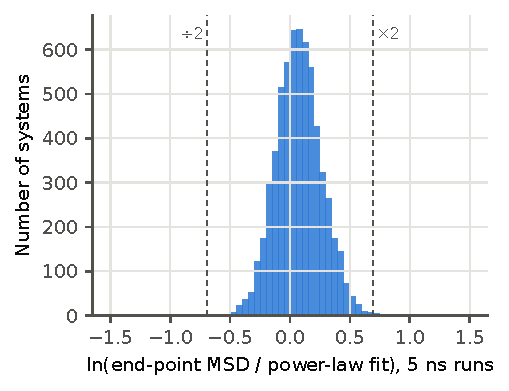
\includegraphics[width=0.55\textwidth]{figures/fig3_endpoint_noise.pdf}
\caption{Deviation of the end-point MSD of the \SI{5}{\nano\second} runs from the power law
fitted over lags between 20\% and 60\% of the run. Dashed lines mark a factor of two.}
\label{si:fig:endpoint}
\end{figure}

\section{Paired short and long runs}\label{si:sec:pairs}
\begin{figure}[ht]
\centering
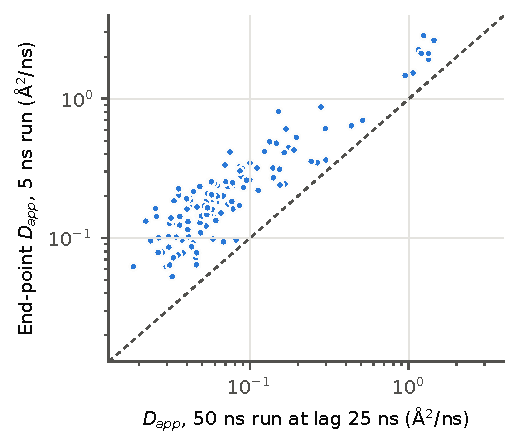
\includegraphics[width=0.5\textwidth]{figures/fig4_short_vs_long.pdf}
\caption{End-point apparent diffusivity from the \SI{5}{\nano\second} run against the
origin-averaged apparent diffusivity at a lag of \SI{25}{\nano\second} from the
\SI{50}{\nano\second} run of the same system, which starts from the same initial structure
(\nPairs{} systems). The dashed line is the identity.}
\label{si:fig:pairs}
\end{figure}

\section{Prefix-based estimators and stopping rules}\label{si:sec:prefix}
\begin{table}[ht]
\centering
\caption{Estimates from a prefix of length $T$ relative to the reference
$\Dapp(\SI{25}{\nano\second})$ of the full \SI{50}{\nano\second} run: median ratio and typical
multiplicative error (\nPrefix{} runs).}\label{si:tab:prefix}
\resizebox{\textwidth}{!}{% Generado por analizar_prefijos.py. No editar a mano.
\begin{tabular}{rrrrrrrrr}
\toprule
 & \multicolumn{2}{c}{End-point} & \multicolumn{2}{c}{Half-lag} & \multicolumn{2}{c}{Linear fit} & \multicolumn{2}{c}{Power-law extrapolation} \\
\cmidrule(lr){2-3}\cmidrule(lr){4-5}\cmidrule(lr){6-7}\cmidrule(lr){8-9}
$T$ (ns) & Ratio & Error & Ratio & Error & Ratio & Error & Ratio & Error \\
\midrule
1 & 6.56 & $\times$6.56 & 10.34 & $\times$10.34 & 3.22 & $\times$3.27 & 0.53 & $\times$1.87 \\
2 & 4.43 & $\times$4.43 & 6.39 & $\times$6.39 & 2.83 & $\times$2.85 & 0.72 & $\times$1.50 \\
5 & 2.83 & $\times$2.83 & 4.05 & $\times$4.05 & 2.02 & $\times$2.02 & 0.95 & $\times$1.37 \\
10 & 2.02 & $\times$2.02 & 2.55 & $\times$2.55 & 1.48 & $\times$1.51 & 1.07 & $\times$1.26 \\
20 & 1.43 & $\times$1.45 & 1.78 & $\times$1.78 & 1.16 & $\times$1.24 & 1.11 & $\times$1.20 \\
30 & 1.20 & $\times$1.23 & 1.38 & $\times$1.38 & 0.95 & $\times$1.20 & 1.05 & $\times$1.13 \\
50 & 0.89 & $\times$1.13 & 1.00 & $\times$1.00 & 0.73 & $\times$1.37 & 0.97 & $\times$1.03 \\
\bottomrule
\end{tabular}
}
\end{table}

\begin{table}[ht]
\centering
\caption{Sensitivity of the prefix-based comparison to the reference (\refN{} long runs). Each
cell gives the typical multiplicative error and, in parentheses, the median ratio of the estimate
to the reference. The power law is extrapolated to the quantity that defines each reference: the
apparent diffusivity at that lag, or the mean slope of $A\tau^{\beta}$ over
20 to \SI{40}{\nano\second}.}\label{si:tab:sens-prefix-ref}
\resizebox{\textwidth}{!}{% Generado por referencias.py. No editar a mano.
\begin{tabular}{lrrrr}
\toprule
Reference (from the 50 ns run) & End-point, 5 ns & Linear fit, 5 ns & Power law, 5 ns & Power law, 10 ns \\
\midrule
$D_{app}$ at 15 ns & $\times$2.37 (2.37) & $\times$1.80 (1.73) & $\times$1.33 (1.06) & $\times$1.22 (1.16) \\
$D_{app}$ at 25 ns (main) & $\times$2.83 (2.83) & $\times$2.02 (2.02) & $\times$1.37 (0.95) & $\times$1.26 (1.07) \\
$D_{app}$ at 35 ns & $\times$3.15 (3.15) & $\times$2.23 (2.23) & $\times$1.39 (0.86) & $\times$1.32 (1.00) \\
$D_{app}$ at 40 ns & $\times$3.27 (3.27) & $\times$2.33 (2.33) & $\times$1.45 (0.83) & $\times$1.30 (0.95) \\
Slope of MSD, 20 to 40 ns & $\times$4.01 (4.01) & $\times$3.05 (3.05) & $\times$1.99 (0.54) & $\times$1.52 (0.68) \\
\bottomrule
\end{tabular}
}
\end{table}

\begin{table}[ht]
\centering
\caption{Stopping rules evaluated on the long runs (\nPrefix{} runs). Runs that do not meet a
rule before \SI{50}{\nano\second} are simulated for the full length and evaluated there. Mean
time and the first error column are averaged over all runs; the last column restricts the error
to the runs that stop early.}\label{si:tab:rules}
\resizebox{\textwidth}{!}{% Generado por analizar_prefijos.py. No editar a mano.
\begin{tabular}{llrrrr}
\toprule
Rule & Estimator & Stop before \SI{50}{\nano\second} & Mean time (ns) & Error, all runs & Error, runs that stop \\
\midrule
Regime: $\beta\ge0.9$ & Linear fit & 3\% & 49.3 & $\times$1.37 & $\times$1.38 \\
Regime: $\beta\ge0.8$ & Linear fit & 19\% & 44.6 & $\times$1.39 & $\times$1.39 \\
Precision: CV $<10\%$ & Linear fit & 2\% & 49.3 & $\times$1.37 & $\times$1.36 \\
Precision: CV $<20\%$ & Linear fit & 80\% & 15.6 & $\times$1.79 & $\times$2.22 \\
Precision: CV $<10\%$ & Power law & 24\% & 43.4 & $\times$1.04 & $\times$1.13 \\
\midrule
Fixed \SI{5}{\nano\second} & End-point & n/a & 5.0 & $\times$2.83 & n/a \\
Fixed \SI{5}{\nano\second} & Linear fit & n/a & 5.0 & $\times$2.02 & n/a \\
Fixed \SI{10}{\nano\second} & Linear fit & n/a & 10.0 & $\times$1.51 & n/a \\
Fixed \SI{20}{\nano\second} & Linear fit & n/a & 20.0 & $\times$1.24 & n/a \\
Fixed \SI{5}{\nano\second} & Power law & n/a & 5.0 & $\times$1.37 & n/a \\
Fixed \SI{10}{\nano\second} & Power law & n/a & 10.0 & $\times$1.26 & n/a \\
Fixed \SI{20}{\nano\second} & Power law & n/a & 20.0 & $\times$1.20 & n/a \\
\bottomrule
\end{tabular}
}
\end{table}

The regime rules rarely fire: the effective exponent of a prefix reaches 0.9 before
\SI{50}{\nano\second} in \ruleBetaNineStopPct\% of the runs and 0.8 in \ruleBetaEightStopPct\%,
so they save almost no simulation, and when the $\beta\ge0.8$ rule fires the error of the runs
that stop is \ruleBetaEightErrStop. The precision rule with a 20\% tolerance stops early in
\ruleCvTwentyStopPct\% of the runs but with a typical error of \ruleCvTwentyErrStop{} for those
runs: a small bootstrap CV measures the precision of a lag-dependent quantity, not its distance
from the long-lag value.

\begin{table}[ht]
\centering
\caption{Settings chosen on half of the systems and evaluated on the other half (median over
\frSplits{} random partitions): mean simulated time, typical error, and percentage of partitions
in which the held-out half meets the target. A dash means that no setting met the target on the
half used for the choice.}\label{si:tab:frontier}
\resizebox{\textwidth}{!}{% Generado por frontera.py. No editar a mano.
\begin{tabular}{lrrrrrr}
\toprule
 & \multicolumn{3}{c}{Target error $\times1.5$} & \multicolumn{3}{c}{Target error $\times1.3$} \\
Rule & Time (ns) & Error & Target met & Time (ns) & Error & Target met \\
\midrule
Fixed length, end-point & 20.0 & $\times$1.45 & 97\% & 30.0 & $\times$1.23 & 84\% \\
Fixed length, linear fit & 12.0 & $\times$1.47 & 61\% & 20.0 & $\times$1.24 & 96\% \\
Fixed length, power law & 2.0 & $\times$1.50 & 59\% & 7.5 & $\times$1.31 & 45\% \\
Regime rule, linear fit & 35.2 & $\times$1.48 & 64\% & n/a & n/a & 0\% \\
Precision rule, linear fit & 37.0 & $\times$1.47 & 67\% & 50.0 & $\times$1.40 & 0\% \\
Precision rule, power law & 11.9 & $\times$1.43 & 76\% & 20.9 & $\times$1.18 & 93\% \\
\bottomrule
\end{tabular}
}
\end{table}

\section{Robustness of the adaptive allocation}\label{si:sec:alloc}
\begin{table}[ht]
\centering
\caption{Mean number of \SI{5}{\nano\second} runs per candidate that boundary-focused allocation
needs to match the recall of uniform replicates, and the corresponding saving (end-point label,
Gaussian system values, \alReps{} simulated campaigns of \alN{} candidates).}\label{si:tab:alloc-eq}
\begin{tabular}{lrrr}
\toprule
 & \multicolumn{3}{c}{Uniform replicates matched} \\
\cmidrule(lr){2-4}
Target & 2 runs & 3 runs & 4 runs \\
\midrule
Top 1\%  & \alEqTopOneUnifTwo{} ($\times$\alSavingTopOneUnifTwo) & \alEqTopOneUnifThree{} ($\times$\alSavingTopOneUnifThree) & \alEqTopOneUnifFour{} ($\times$\alSavingTopOneUnifFour) \\
Top 5\%  & \alEqTopFiveUnifTwo{} ($\times$\alSavingTopFiveUnifTwo) & \alEqTopFiveUnifThree{} ($\times$\alSavingTopFiveUnifThree) & \alEqTopFiveUnifFour{} ($\times$\alSavingTopFiveUnifFour) \\
Top 10\% & \alEqTopTenUnifTwo{} ($\times$\alSavingTopTenUnifTwo) & \alEqTopTenUnifThree{} ($\times$\alSavingTopTenUnifThree) & \alEqTopTenUnifFour{} ($\times$\alSavingTopTenUnifFour) \\
\bottomrule
\end{tabular}
\end{table}

The saving for the top 10\% against four uniform replicates is $\times$\alSavingTopTenUnifFourEmpEnd{}
when the system values follow the empirical shape of the \nShort{} short runs instead of a normal
distribution, and $\times$\alSavingTopTenUnifFourNormAvg{} with the origin-averaged label. Using
the mobility-dependent noise in the allocation does not help: the recall of the top 10\% with
four runs per candidate is \alBoundTopTenBFour\% with it and \alBoundHomoTopTenBFour\% with a
constant noise.
Successive halving with restarted rounds performs similarly to boundary-focused allocation. With
the end-point label and 1.25 runs per candidate it recovers \alHalvingTopOneBOneQuarterEnd\% of the top 1\%,
against \alBoundTopOneBOneQuarterEnd\%; with the origin-averaged label and four runs per candidate it recovers
\alHalvingTopOneBFourAvg\%, against \alBoundTopOneBFourAvg\%.

\section{Check of the adaptive allocation on real runs}\label{si:sec:val-alloc}
\begin{table}[ht]
\centering
\caption{Check of the adaptive allocation on the replicated systems. Calibration: \valAlNRep{}
systems, predictions in both directions (first run $\to$ second and second $\to$ first), noise
parameters estimated leaving out the system evaluated. Campaign: \valAlNCamp{} systems with a long
run; every system receives its first run and \valAlExtra{} receive a second run, chosen at the
boundary or at random (mean of 2000 draws); recall of the top set according to the long run.
Interval: bootstrap over systems of the difference between boundary and random placement.}
\label{si:tab:val-alloc}
\begin{tabular}{lrr}
\toprule
 & Top 10\% & Top 20\% \\
\midrule
Brier improvement over the base rate & \valAlBrierGainTen\% & \valAlBrierGainTwenty\% \\
Calibration slope (95\% CI) & \valAlCalSlopeTen{} (\valAlCalSlopeLoTen{} to \valAlCalSlopeHiTen) & \valAlCalSlopeTwenty{} (\valAlCalSlopeLoTwenty{} to \valAlCalSlopeHiTwenty) \\
\addlinespace
Systems in the top set, $k$ & \valAlKTen & \valAlKTwenty \\
Recall, first runs only & \valAlOnlyATen\% & \valAlOnlyATwenty\% \\
Recall, second runs at random & \valAlRandomTen\% & \valAlRandomTwenty\% \\
Recall, second runs at the boundary & \valAlBoundTen\% & \valAlBoundTwenty\% \\
Recall, second runs for all & \valAlBothTen\% & \valAlBothTwenty\% \\
Boundary $-$ random (95\% CI, points) & $\valAlDiffLoTen$ to $+\valAlDiffHiTen$ & $\valAlDiffLoTwenty$ to $+\valAlDiffHiTwenty$ \\
\bottomrule
\end{tabular}
\end{table}

The long runs start from the same structure as the first runs, so they favour the first run and
understate the value of any second run from a new structure; this is why no strategy improves on
the first run alone for the top 20\%, and why the check is conservative.

\end{document}
